\documentclass[preprint,12pt,authoryear]{elsarticle}
\usepackage[letterpaper,hmargin=0.9in,top=0.76in,bottom=0.78in]{geometry}
\usepackage[T1]{fontenc}
\usepackage{lmodern,textcomp}
\usepackage{xcolor}
\usepackage{booktabs,tabularx,array}
\usepackage{flafter}
\usepackage{needspace}
\usepackage{capt-of}
\usepackage{listings}
\usepackage{tikz}
\usepackage{tcolorbox}
\tcbuselibrary{breakable}
\usepackage[hidelinks]{hyperref}

% ============================================================
% References to the main paper: edit here if its numbering changes
% ============================================================
\newcommand{\papertitle}{A Neuro-Symbolic Architecture for Safe and Feasible Self-Recovery in Multi-Agent Manufacturing Systems}
\newcommand{\FigOutline}{Fig.~5}
\newcommand{\FigComposition}{Fig.~6}

% ============================================================
% Page and heading style (as in the template)
% ============================================================
\pagestyle{plain}
\setlength{\parindent}{0pt}
\setlength{\parskip}{4pt}
\raggedbottom
\emergencystretch=2em
\setlength{\textfloatsep}{10pt plus 2pt minus 2pt}
\setlength{\intextsep}{8pt plus 2pt minus 2pt}
\setlength{\abovecaptionskip}{4pt}
\setlength{\belowcaptionskip}{0pt}
\makeatletter
\renewcommand\section{\@startsection{section}{1}{\z@}%
  {14pt plus 4pt minus 2pt}{6pt plus 2pt minus 2pt}{\large\bfseries\boldmath}}
\renewcommand\subsection{\@startsection{subsection}{2}{\z@}%
  {10pt plus 3pt minus 2pt}{3pt plus 1pt minus 1pt}{\normalsize\bfseries}}
% On a page that holds only tables, they start at the top with a fixed gap between them.
\setlength{\@fptop}{0pt}
\setlength{\@fpsep}{12pt}
\setlength{\@fpbot}{0pt plus 1fil}
\makeatother

% ============================================================
% Text styles. Two families only: the serif text face, and one monospaced
% face for names and for text copied from the records.
%   body                      12 pt serif
%   tables, captions, key     \footnotesize serif
%   recorded text             9 pt monospaced, in boxes and in table cells
%   labels inside boxes       9 pt serif bold (ours, not recorded)
%   notes on omitted lines    9 pt serif italic, gray (ours)
% Colour is used only for the pass and fail marks, the red bar, and the figure.
% ============================================================
\definecolor{markgreen}{RGB}{56,118,29}
\definecolor{markred}{RGB}{192,0,0}
\definecolor{cutgray}{gray}{0.40}

\lstdefinestyle{record}{
  basicstyle=\fontsize{9}{11}\selectfont\ttfamily,
  columns=fullflexible, keepspaces=true, showstringspaces=false, upquote=true,
  breaklines=true, breakatwhitespace=true, breakindent=9.5pt, breakautoindent=true,
  prebreak={}, postbreak={},
  aboveskip=0pt, belowskip=0pt,
  escapeinside={(*@}{@*)}
}
\lstset{style=record}

% A cut inside a recorded line, and recorded lines left out.
\newcommand{\cut}{{\normalfont\ttfamily\color{cutgray}[...]}}
\newcommand{\vd}{\raisebox{-0.1ex}{\vbox{\baselineskip 3pt\lineskip 0pt\lineskiplimit 0pt\hbox{.}\hbox{.}\hbox{.}}}}
\newcommand{\skipped}[1]{{\normalfont\itshape\fontsize{9}{11}\selectfont\color{cutgray}\vd\enspace #1}}
% A recorded name inside one of our notes or labels: plain monospaced, in the colour of the note.
\newcommand{\secname}[1]{{\normalfont\ttfamily #1}}
% Who wrote the lines that follow (our label, not recorded text).
\newcommand{\who}[1]{{\normalfont\bfseries\fontsize{9}{11}\selectfont\rule{0pt}{2.6ex}#1}}
% A bar in the margin beside the line to notice.
\newcommand{\notebar}{\rlap{\hspace{-5pt}\textcolor{markred}{\rule[-0.35ex]{2pt}{1.9ex}}}}
% Recorded text inside a table cell.
\newcommand{\rec}[1]{{\fontsize{9}{11}\selectfont\ttfamily\frenchspacing #1}}

% Names from the records in running text: the monospaced text face itself,
% so every character comes from one font. A line may break after a slash only.
% They are set slightly smaller than the text around them, so that the two faces look the same size.
\makeatletter
\newcommand{\codesize}{\fontsize{\dimexpr\f@size pt*92/100\relax}{\f@baselineskip}\selectfont}
\DeclareRobustCommand{\code}[1]{{\codesize\ttfamily\frenchspacing\expandafter\code@scan\detokenize{#1}\code@end}}
\def\code@scan#1{\ifx#1\code@end\else\code@put#1\expandafter\code@scan\fi}
\def\code@put#1{#1\ifnum`#1=`\/ \penalty\exhyphenpenalty\fi}
\let\code@end\relax
\makeatother

% Verdict marks, drawn so that they look the same in every engine.
\newcommand{\ok}{\tikz[baseline=-0.55ex]{\draw[line width=0.9pt, color=markgreen!80!black, line cap=round, line join=round] (0,0) -- (0.08,-0.09) -- (0.24,0.12);}}
\newcommand{\no}{\tikz[baseline=-0.55ex]{\draw[line width=0.9pt, color=markred, line cap=round] (0,-0.09) -- (0.19,0.11) (0,0.11) -- (0.19,-0.09);}}
\newcommand{\na}{--}

% ============================================================
% Gray titled boxes (as in the template). recbox never breaks across a page;
% fullbox is used once, for the complete prompt in Appendix D, which runs over four pages.
% ============================================================
\tcbset{recstyle/.style={colback=black!2, colframe=black!40, colbacktitle=black!10, coltitle=black,
  arc=4pt, boxrule=0.4pt, left=7pt, right=7pt, top=5pt, bottom=5pt, fonttitle=\small\bfseries}}
\newtcolorbox{recbox}[1]{recstyle, title={#1}, before skip=2pt, after skip=3pt}
\newtcolorbox{fullbox}[1]{recstyle, breakable, title={#1},
  title after break={#1 (continued)}, before skip=2pt, after skip=3pt}

\newcolumntype{Y}{>{\raggedright\arraybackslash}X}

\begin{document}

\begin{center}
  {\Large\bfseries \papertitle\par}
  \medskip
  {\large Supplementary Material\par}
\end{center}

This supplement follows one recovery from the experiments, Part slippage, from the failure to
robot motion. Appendix~A shows how the recovery outline was synthesized: the large language
model (LLM) proposed one event at a time, and each event was accepted only after checks by the
Resource Agent (RA) and the Central Controller Agent (CCA) (\FigOutline{} of the paper).
Appendix~B shows how one accepted event was composed from robot primitives (\FigComposition).
Appendix~C reports the run of the composed programs in Gazebo. Appendix~D is reference
material: one candidate event in full, what differs in the other experimental settings, and
the complete first prompt. The run uses the framework at the event level, where the LLM
proposes candidates for one event at a time, with Claude Opus~5.5 at medium reasoning effort.

\appendix
\renewcommand{\thesection}{Appendix~\Alph{section}}
\renewcommand{\thesubsection}{\Alph{section}.\arabic{subsection}}
\makeatletter
\@addtoreset{table}{section}
\@addtoreset{figure}{section}
\makeatother
\renewcommand{\theHtable}{\Alph{section}.\arabic{table}}
\renewcommand{\theHfigure}{\Alph{section}.\arabic{figure}}

% ============================================================
\section{Recovery Outline Synthesis}\label{sec:outline}
% ============================================================

\subsection{The failure}

In the Gazebo simulation of the cell, the failure is injected while robot \code{ur5e-4} lowers
the small gear onto the assembly board: its gripper opens, and the gear is put on the table at
a set position, at no station. The robot stops above the board, and a fault is reported. Robot
\code{ur5e-3} is at the buffer with the square peg in its gripper (Fig.~\ref{fig:scene}).

\begin{figure}[!htb]
\centering
\begin{minipage}[c]{0.47\linewidth}
\centering
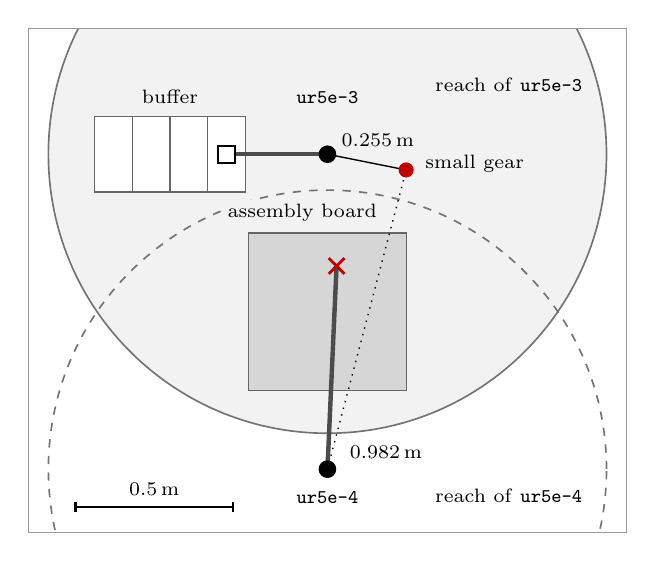
\begin{tikzpicture}[x=4.0cm,y=4.0cm,font=\scriptsize]
  \begin{scope}
    \clip (-0.95,-0.70) rectangle (0.95,0.90);
    % reach of ur5e-3 (solid, shaded) and of ur5e-4 (dashed)
    \fill[black!5] (0,0.5) circle [radius=0.886];
    \draw[black!55, line width=0.6pt] (0,0.5) circle [radius=0.886];
    \draw[black!55, line width=0.6pt, dashed] (0,-0.5) circle [radius=0.886];
    % assembly board area and the four buffer zones
    \fill[black!16] (-0.25,-0.25) rectangle (0.25,0.25);
    \draw[black!60] (-0.25,-0.25) rectangle (0.25,0.25);
    \fill[white] (-0.74,0.38) rectangle (-0.26,0.62);
    \draw[black!60] (-0.74,0.38) rectangle (-0.26,0.62);
    \draw[black!60] (-0.62,0.38) -- (-0.62,0.62) (-0.50,0.38) -- (-0.50,0.62) (-0.38,0.38) -- (-0.38,0.62);
  \end{scope}
  \draw[black!40] (-0.95,-0.70) rectangle (0.95,0.90);
  % the two distances to the gear
  \draw[black, line width=0.5pt] (0,0.5) -- (0.25,0.45);
  \draw[black, line width=0.5pt, dotted] (0,-0.5) -- (0.25,0.45);
  % arms, from base to gripper
  \draw[line width=1.6pt, black!70] (0,0.5) -- (-0.32,0.5);
  \draw[line width=1.6pt, black!70] (0,-0.5) -- (0.029,0.145);
  \fill (0,0.5) circle [radius=0.028];
  \fill (0,-0.5) circle [radius=0.028];
  % gripper of ur5e-3 with the square peg; gripper of ur5e-4 over the gear's slot
  \filldraw[fill=white, draw=black, line width=0.6pt] (-0.347,0.473) rectangle (-0.293,0.527);
  \draw[markred, line width=1pt] (0.004,0.120) -- (0.054,0.170) (0.004,0.170) -- (0.054,0.120);
  % the fallen gear
  \fill[markred] (0.25,0.45) circle [radius=0.024];
  % labels
  \node[anchor=south] at (0,0.63) {\texttt{ur5e-3}};
  \node[anchor=north] at (0,-0.54) {\texttt{ur5e-4}};
  \node[anchor=south] at (-0.50,0.63) {buffer};
  \node[anchor=south, fill=black!5, inner sep=1.5pt] at (-0.08,0.272) {assembly board};
  \node[anchor=west] at (0.28,0.47) {small gear};
  \node[anchor=south] at (0.16,0.495) {0.255\,m};
  \node[anchor=west] at (0.04,-0.445) {0.982\,m};
  \node[anchor=east] at (0.84,0.72) {reach of \texttt{ur5e-3}};
  \node[anchor=east] at (0.84,-0.585) {reach of \texttt{ur5e-4}};
  % scale bar
  \draw[line width=0.8pt] (-0.80,-0.62) -- (-0.30,-0.62);
  \draw[line width=0.8pt] (-0.80,-0.635) -- (-0.80,-0.605) (-0.30,-0.635) -- (-0.30,-0.605);
  \node[anchor=south] at (-0.55,-0.615) {0.5\,m};
\end{tikzpicture}
\end{minipage}\hfill
\begin{minipage}[c]{0.50\linewidth}
\footnotesize\raggedright
The dot is the small gear. It lies on the table, 0.255\,m from the base of \code{ur5e-3}
and 0.982\,m from the base of \code{ur5e-4}. The solid and the dashed circle are the
horizontal limits of the two arms' declared work envelopes, 0.886\,m from each base, so of
the two arms only \code{ur5e-3} can reach the gear.\par\smallskip
The square is the gripper of \code{ur5e-3}, above the buffer and holding the square
peg.\par\smallskip
The cross is the gripper of \code{ur5e-4}. It stopped inside the board area, where only one
resource may be at a time.
\end{minipage}
\caption{The cell at the failure, seen from above: our drawing, to scale, from the recorded
positions. Each arm is drawn as a straight line from its base to its gripper; its joints are
not shown. The first prompt
gives the LLM the measured positions of the gear and of the two grippers; the distances reach
it in turn~2, on its request.}
\label{fig:scene}
\end{figure}

The state of the cell at this moment was recorded. The outline and the programs of
Appendices~A and~B are made from that record, without the simulator; Appendix~C replays the
programs in a new simulation. In this run the recovery frees the gripper of \code{ur5e-3},
moves \code{ur5e-4} away from the board, and has \code{ur5e-3} pick up the gear and place it.
The LLM is given the measurements, not this plan.

\subsection{What the LLM is given}

Table~\ref{tab:prompt} shows the first prompt of the run. Its Failure and Recovery Goal
sections are printed in full. The other five sections are folded to one line each;
Appendix~D prints them in full.

In this and the other gray boxes, monospaced text is copied from the records; only its line
breaks and indentation are ours. A bold line says who wrote the lines under it, a gray \cut{}
marks a cut inside a line, and three gray dots with a note mark lines left out. Every prompt
and reply of the run is in the supplementary files, in \code{transcripts/part_slippage/}.

\begin{table}[!htb]
\begin{recbox}{Outline prompt, turn 1}
% begin recorded prompt-t1
\begin{lstlisting}
(*@\skipped{\secname{Task and Role}: 3 lines, which ask for a plan and for 2 to 5 candidate events for its next step}@*)
Failure
What was detected and measured, stated the same way for every resource.
- ur5e-4 did not complete place_approach of gear_small (destination_location assembly_board-v1)
- task_outcome (ur5e-4, task environment_9): goal_cancelled true, terminal_status 5, progress 0.503
- device_fault_report (ur5e-4): resource_state failed, reported_by gripper object detection
- state_discrepancy (ur5e-4, gear_small): expected_holder ur5e-4, measured_holder null
- gear_small: not held, not at any station, measured at (0.250, 0.450, 1.025)
- ur5e-4: measured pose (0.029, 0.145, 1.289), inside assembly_board-v1

Recovery Goal
- gear_small: part_location assembly_board-v1 (target Gear_Plate/Gear_Shaft_1) (normally ur5e-4's place_insert; ur5e-4 failed)
(*@\skipped{\secname{Candidate Rules}: 7 rules on how to write a recovery event}@*)
(*@\skipped{\secname{Knowledge Base}: 11 references to facts the LLM may ask for}@*)
(*@\skipped{\secname{Resources}: 12 entries, one per resource, with its recorded state and what it can do; one of them:}@*)
ur5e-3 (robot)  picked; held_part KET4_Square_4mm; resource_location Buffer For Machined parts; (*@\cut@*) actions: compute_pick_targets; compute_place_targets; (*@\cut@*)
(*@\skipped{\secname{Parts}: 12 entries, one per part, with its location and state}@*)
\end{lstlisting}
% end recorded prompt-t1
\end{recbox}
\caption{The first prompt of the run, with five of its seven sections folded (\texttt{outline.md}, turn 1).}\label{tab:prompt}
\end{table}

The Failure section reports that \code{ur5e-4} did not finish its move, that it no longer
holds the small gear (\code{gear_small}), and where the gear and the arm were measured. The
Recovery Goal is one line: the gear on the assembly board, at its slot. The entry of
\code{ur5e-3} says that it holds the square peg (\code{KET4_Square_4mm}). The prompt does not
say which robot should fetch the gear, that \code{ur5e-3} must first put down the peg, or that
\code{ur5e-4} must leave the board. It also has no section of safety rules.

\subsection{The run, turn by turn}

The Product Agent sends the prompt. In each turn the LLM replies with a short plan and does
one of three things: it asks for facts, it proposes two to five candidates for the next event
in its order of preference, or it declares the recovery complete. The RA checks the candidates in that
order for feasibility: whether the resource can bring about the stated end state with the
primitives its model declares and within its reach. The CCA checks each feasible candidate against the
safety rules. The first candidate that passes both checks becomes the next recovery event; a
refused one comes back in the next prompt with the reason. Accepted events are planned, not
executed: no robot moves until Appendix~C. Table~\ref{tab:ledger} is the whole run.

\begin{table}[!htb]
\centering\footnotesize
\setlength{\tabcolsep}{4pt}
\begin{tabularx}{\linewidth}{@{}c Y l l l@{}}
\toprule
Turn & LLM reply & RA feasibility & CCA & Result \\
\midrule
1 & Asks for 8 facts, among them how far the gear is from each arm & \na & \na & facts added \\
 & \multicolumn{4}{p{\dimexpr\linewidth-1.2cm\relax}@{}}{\raggedright\textbf{Answer in the next prompt, in part:} \rec{"ur5e-3": \{"max\_xy\_radius\_m": 0.886, \cut{} "xy\_distance\_m": 0.255, \cut{}\}, "ur5e-4": \{"max\_xy\_radius\_m": 0.886, \cut{} "xy\_distance\_m": 0.982, \cut{}\}}} \\
\addlinespace[2pt]
2 & Place the square peg on the board: \code{place_KET4_on_assembly_board} (\code{ur5e-3}) & \ok\ \code{FEASIBLE} & \no\ \code{UNSAFE} & refused \\
 & \multicolumn{4}{p{\dimexpr\linewidth-1.2cm\relax}@{}}{\raggedright\textbf{Reason from the CCA:} \rec{SAFE\_shared\_area\_mutex (At most one resource may occupy the assembly\_board-v1 destination area at any time.) is broken during the event: ur5e-3 is in assembly\_board-v1 while ur5e-4 is in assembly\_board-v1}} \\
2 & Put the square peg in the buffer: \code{stage_KET4_in_buffer} (\code{ur5e-3}) & \ok\ \code{FEASIBLE} & \ok\ \code{SAFE} & event 1 \\
\addlinespace[2pt]
3 & Send \code{ur5e-4} home: \code{retract_ur5e4_home_clear_board} (\code{ur5e-4}) & \ok\ \code{FEASIBLE} & \ok\ \code{SAFE} & event 2 \\
\addlinespace[2pt]
4 & Pick up the gear, stating a pose: \code{pick_dropped_gear_small_ur5e3} (\code{ur5e-3}) & \no\ \code{INFEASIBLE} & \na & refused \\
 & \multicolumn{4}{p{\dimexpr\linewidth-1.2cm\relax}@{}}{\raggedright\textbf{Reason from the RA:} \rec{gear\_small\textquotesingle{}s recorded position gives ur5e-3\textquotesingle{}s target, so this event takes no pose; it states \{x:~0.250, y:~0.450, z:~1.243\}}} \\
4 & The same with a pose 10\,mm higher, refused for the same reason: \code{pick_dropped_gear_small_ur5e3_grip_center} (\code{ur5e-3}) & \no\ \code{INFEASIBLE} & \na & refused \\
\addlinespace[2pt]
5 & Pick up the gear, no pose: \code{pick_dropped_gear_small_ur5e3} (\code{ur5e-3}) & \ok\ \code{FEASIBLE} & \ok\ \code{SAFE} & event 3 \\
\addlinespace[2pt]
6 & Place the gear in its slot: \code{place_gear_small_on_board_ur5e3} (\code{ur5e-3}) & \ok\ \code{FEASIBLE} & \ok\ \code{SAFE} & event 4 \\
\addlinespace[2pt]
7 & Declares the recovery complete & \na & \ok\ \code{NONBLOCKING} & accepted \\
\bottomrule
\end{tabularx}
\caption{Outline synthesis for Part slippage: 7 turns, 8 facts looked up, 4 accepted events, 68,402 tokens of input and output. A dash means that the check was not run. In turns 2, 3, 5 and 6 the last candidate, ranked after the accepted one, was not checked and is not listed.}\label{tab:ledger}
\end{table}

\subsection{How feedback changed the outline}

Table~\ref{tab:cca} follows the first refusal through three records. In turn~2 the LLM's first
choice was to place the square peg on the board. The RA found this feasible. The CCA refused
it, because \code{ur5e-4} was still in the board area. The reason came back in the prompt of
turn~3. This is the first time the LLM reads a safety rule: the name and the wording of the
one its candidate broke. Its next plan begins by sending \code{ur5e-4} home.

\begin{table}[!htb]
\begin{recbox}{Turns 2 and 3: a candidate refused by the CCA}
% begin recorded cca-refusal
\begin{lstlisting}
(*@\who{LLM reply, turn 2: its plan and its first candidate}@*)
{"plan": "gear_small is outside ur5e-4's work envelope but inside ur5e-3's, so ur5e-3 must recover it, and its gripper is still holding KET4_Square_4mm. First ur5e-3 puts down KET4, then it picks gear_small and places it on assembly_board-v1 at Gear_Plate/Gear_Shaft_1.",
(*@\cut@*) "event_name": "place_KET4_on_assembly_board",
(*@\skipped{the rest of this candidate, and two more candidates (Appendix D prints the second in full)}@*)
(*@\who{Prompt, turn 3: the section added after the refusal}@*)
Validation Feedback
These candidates were refused, and stage_KET4_in_buffer, listed after them, was applied.
- candidate_event=c1/ur5e-3/KET4_Square_4mm | event_name=place_KET4_on_assembly_board | constraint_code=cca_safety | reason=SAFE_shared_area_mutex (At most one resource may occupy the assembly_board-v1 destination area at any time.) is broken during the event: ur5e-3 is in assembly_board-v1 while ur5e-4 is in assembly_board-v1
(*@\who{LLM reply, turn 3: its plan}@*)
{"plan": "ur5e-4 is failed and still occupies the assembly_board-v1 area, which blocks ur5e-3, so first clear it by sending ur5e-4 home. Then ur5e-3, whose envelope contains gear_small, picks the gear and inserts it at Gear_Plate/Gear_Shaft_1 on assembly_board-v1.",
(*@\skipped{two candidates, of which the first became event 2}@*)
\end{lstlisting}
% end recorded cca-refusal
\end{recbox}
\caption{A safety refusal: the proposal, the feedback in the next prompt, and the next plan (\texttt{outline.md}, turns 2 and 3).}\label{tab:cca}
\end{table}

The second candidate of turn~2, putting the peg in the buffer, passed both checks and became
event~1. Sending \code{ur5e-4} home became event~2. That robot is in the state \code{failed},
a fault reported by its gripper; the RA found that it can still make this move.

Table~\ref{tab:ra} follows the second refusal. In turn~4 the LLM proposed to pick up the gear
and wrote a position for the arm into the intended end state of the event
(\code{expected_end_state}). A rule of the prompt allows a position only where nothing else
gives it, and \code{ur5e-3} declares the primitive \code{compute_pick_targets}, which
calculates its pick target from the gear's recorded position. The pose was refused for being stated: the RA does not judge its value, and
it found the pick itself reachable. \code{INFEASIBLE} is the RA's word for any refusal.

\begin{table}[!htb]
\begin{recbox}{Turns 4 and 5: a candidate refused by the RA}
% begin recorded ra-refusal
\begin{lstlisting}
(*@\who{Prompt, every turn: part of the third Candidate Rule}@*)
(*@\cut@*) Give `pose` only for a position nothing else gives: an arm's pick or place target comes from the part or the place when it declares compute_pick_targets or compute_place_targets, (*@\cut@*)
\end{lstlisting}

\vspace{3pt}{\color{black!30}\hrule height 0.3pt}\vspace{3pt}
\begin{minipage}[t]{0.485\linewidth}
\begin{lstlisting}
(*@\who{LLM reply, turn 4: first candidate, refused}@*)
(*@\cut@*) "expected_end_state": {
  "held_part": "gear_small",
  "resource_state": "picked",
  "resource_location": null,
(*@\notebar@*)  "pose": {"x": 0.25, "y": 0.45, "z": 1.243},
  "part_location": "ur5e-3"
}, (*@\cut@*)
\end{lstlisting}
\end{minipage}\hfill
\begin{minipage}[t]{0.485\linewidth}
\begin{lstlisting}
(*@\who{LLM reply, turn 5: first candidate, accepted}@*)
(*@\cut@*) "expected_end_state": {
  "resource_state": "picked",
  "held_part": "gear_small",
  "resource_location": null,
  "part_location": "ur5e-3"
}, (*@\cut@*)
\end{lstlisting}
\end{minipage}

\vspace{3pt}{\color{black!30}\hrule height 0.3pt}\vspace{3pt}
\begin{lstlisting}
(*@\who{Prompt, turn 5: the section added after the refusal}@*)
Validation Feedback
- candidate_event=RECOVERY_SEQ3/ur5e-3/gear_small | event_name=pick_dropped_gear_small_ur5e3 | constraint_code=ra_feasibility | reason=gear_small's recorded position gives ur5e-3's target, so this event takes no pose; it states {x: 0.250, y: 0.450, z: 1.243}
(*@\skipped{one more line, with the same reason for the second candidate, which states a height of 1.253}@*)
\end{lstlisting}
% end recorded ra-refusal
\end{recbox}
\caption{A feasibility refusal: the rule, the end state before and after, and the feedback between them. The red bar marks the stated pose (\texttt{outline.md}, turns 4 and 5).}\label{tab:ra}
\end{table}

\needspace{5\baselineskip}
In turn~6 the LLM proposed to place the gear in its slot, which became event~4, and in
turn~7 it declared the recovery complete. The CCA then checked that the outline is
nonblocking: from the state the four events leave, however the running tasks complete, the
square peg can still reach its assembly and the robots in the check's model can still return
to rest. The outline of four events, $s^R = e^R_1 e^R_2 e^R_3 e^R_4$, was accepted.

\subsection{Notes on this run}

Three facts qualify these results.
\begin{itemize}\setlength{\itemsep}{2pt}\setlength{\parskip}{0pt}\setlength{\topsep}{2pt}
\item The run was chosen as follows. Among the passing event-level framework outlines that the
three LLMs produced for this failure in the first run of the experiments, it is one with the
fewest events. That run was made before the model of the resource Exit was corrected (see the
paper). None of the four accepted events uses Exit; the nonblocking check used the Exit model
as it was then.
\item The safety checks rest on one declared assumption: \code{ur5e-3} counts as outside the
board area until an event moves it. The failure was recorded without the CCA, and the
recorded bounds of the upper arm of \code{ur5e-3} then reach over the edge of the board area;
with the CCA on, \code{ur5e-3} would have waited outside.
\item The nonblocking check explored 368 states of a model of the square peg and six
resources: the buffer, Exit, the KMR, \code{ur5e-1}, \code{ur5e-2} and \code{ur5e-3}. The robot
that failed, \code{ur5e-4}, is not in this model, and the safety rules are not part of this
check. The record of the run also lists the normal tasks that follow the outline; three
bookkeeping values that the normal grasp task of \code{ur5e-3} needs are noted there as
assumed, not checked.
\end{itemize}

% ============================================================
\section{Primitive Composition of Event 3}\label{sec:composition}
% ============================================================

Appendix~B follows event~3, picking up the gear (\FigComposition{} of the paper sketches an
event of this kind). For each accepted event the RA prompts the LLM again, this time for a
program of the robot's primitives. The outline has fixed the robot and the intended end state;
the LLM now decides how the robot reaches, grasps and withdraws. Composing the four events
took nine LLM calls, and event~3 took calls 5 to~7. Table~\ref{tab:blocks} lists what the
prompt of call~5 holds.

\begin{table}[!htb]
\centering\footnotesize
\setlength{\tabcolsep}{5pt}
\begin{tabularx}{\linewidth}{@{}>{\raggedright\arraybackslash}p{4.4cm} Y@{}}
\toprule
Block of the prompt & What it holds \\
\midrule
Task and Role & The task, in its words: \rec{Author primitive\_steps for ONLY the active DES transition, using only the visible primitive catalog for the active resource.} \\
Visible Primitive Catalog & The names of the eight primitives of \code{ur5e-3} that a program may use. \\
Published Ref Schema & Fifteen references to facts the LLM may ask for, such as the contract of a primitive (its description and parameters) or the last observed pose of a part. \\
Available Capability Decompositions & The names of five functions of normal production, such as \code{pick_approach}. The LLM may ask how each is built from primitives. \\
Active DES Transition & The accepted event, with its start state and its intended end state. \\
Three short blocks & A cursor, a one-line summary of the event, and the named pose the robot may use (\code{home}). \\
Output Contract & Eight rules for the reply. By one of them every number in a program is a \code{context_ref}, a reference to a value that the RA holds or calculates, so the LLM writes no coordinates. \\
RA composition validation & One paragraph on how the RA checks a program. \\
\bottomrule
\end{tabularx}
\caption{The blocks of the user message of the composition prompt of call 5, in order (\texttt{composition.md}, call 5). A system message fixes the format of the reply.}\label{tab:blocks}
\end{table}

In call~5 the LLM asked for eleven facts, among them the contracts of five primitives, the
gear's recorded pose, and the step lists of \code{pick_approach} and \code{pick_grasp}, two
functions of normal production. In call~6 it submitted a program whose first step passed the
gear's pose into \code{compute_pick_targets}, an optional input of that primitive. The RA
returned one finding
(Table~\ref{tab:revision}). When the RA checks a program it makes this calculation itself from
the recorded observations, with no pose passed in, which is the \code{None} in the finding; an
input that differs from what the calculation reads is refused. In call~7 the LLM passed only
the part name, and the RA accepted the program (Table~\ref{tab:program}).

\begin{table}[!htb]
\begin{recbox}{Composition of event 3, calls 6 and 7: the finding and the revision}
% begin recorded comp-revision
\begin{lstlisting}
(*@\who{LLM reply, call 6: the parameters of step 1, \secname{compute\_pick\_targets}}@*)
(*@\cut@*) "part_name": "gear_small",
"target_pose": {
  "x": {"context_ref": "/parts/gear_small/observed_pose/x"},
(*@\skipped{\secname{y}, \secname{z} and \secname{model\_name}}@*)
},
"target_pose_source": "observed_pose" (*@\cut@*)
(*@\who{Prompt, call 7: the section added after the RA's check}@*)
Previous Validation Feedback (read first)
- RECOVERY_SEQ3 / recovery-resource-3@localhost [composition_missing_context]: compute_pick_targets: target_pose (*@\cut@*) differs from None, the input the composition's calculation reads; compute_pick_targets: target_pose_source 'observed_pose' differs from '', the input the composition's calculation reads
(*@\who{LLM reply, call 7: its rationale, step 1, and the first parameter of step 2}@*)
(*@\cut@*) "rationale": "Following the validation finding, compute_pick_targets no longer receives target_pose or target_pose_source, so the owner calculation reads the recorded pose itself.",
(*@\cut@*) {"primitive": "compute_pick_targets", "params": {"part_name": "gear_small"}},
(*@\cut@*) "x": {"context_ref": "event_facts.pick_targets.gear_small.approach_pose.x"}, (*@\cut@*)
\end{lstlisting}
% end recorded comp-revision
\end{recbox}
\caption{The one revision in the composition of event 3 (\texttt{composition.md}, calls 6 and 7). In these records \texttt{ur5e-3} appears under the address of its agent, \texttt{recovery-resource-3@localhost}; the code in brackets is the check's code for a program it cannot confirm as written.}\label{tab:revision}
\end{table}

\begin{table}[!htb]
\centering\footnotesize
\setlength{\tabcolsep}{5pt}
\begin{tabularx}{\linewidth}{@{}c l Y Y@{}}
\toprule
Step & Primitive & Written by the LLM & Resolved by the RA \\
\midrule
1 & \code{compute_pick_targets} & The part name. & The approach, grasp and retreat poses, calculated from the gear's recorded position. \\
2 & \code{move_cartesian} & A reference to the approach pose. & \mbox{(0.250, 0.450, 1.303)}, above the gear. \\
3 & \code{move_cartesian} & A reference to the grasp pose. & \mbox{(0.250, 0.450, 1.253)}, at the grasp height. \\
4 & \code{grasp_part} & The part name, and its model name by reference. & \code{gear_small}. The gear is then held. \\
5 & \code{move_cartesian} & A reference to the retreat pose. & \mbox{(0.250, 0.450, 1.303)}, withdrawn with the gear. \\
\bottomrule
\end{tabularx}
\caption{The accepted program for event 3. Positions are in metres, rounded to three decimals.}\label{tab:program}
\end{table}

The accepted program follows the step lists of \code{pick_approach} and \code{pick_grasp}
that the LLM had asked for, with three small changes. It leaves out the detection step of
\code{pick_approach}, which that list allows when the part's pose has been retrieved. After
the grasp it reaches the retreat pose with an absolute move, where \code{pick_grasp} uses a
relative lift for a pick like this one, and it passes no speed for that move. The positions are those of the
arm's controlled link, which is 0.218\,m above the tool centre point of the gripper; the
calculation sets that point 0.010\,m above the gear's measured height of 1.025\,m. The RA
checked the five steps
without moving the robot and recorded \code{FEASIBLE}: the program leaves the end state that
the event promised. The CCA checked the event (Appendix~A); it did not check the composed
program. Composing all four events took 144,642 tokens of input and output.

% ============================================================
\section{Execution in Gazebo}\label{sec:gazebo}
% ============================================================

The four composed programs, 16 primitive steps in all, were then replayed in Gazebo. The
failure was first reproduced in the simulation. Each composed step then ran on the robot's
controller, in order, with the values resolved during composition. This run tests the composed programs
only: the CCA does not supervise it, the checks of Appendices~A and~B are not repeated, and it
ends when the fourth event completes, without resuming normal production. An event counts as
completed when each of its motion and gripper steps reports success. All four events
completed (Table~\ref{tab:gazebo}).

\begin{table}[!htb]
\centering\footnotesize
\setlength{\tabcolsep}{5pt}
\begin{tabularx}{\linewidth}{@{}>{\raggedright\arraybackslash}p{3.5cm} Y c >{\raggedright\arraybackslash}p{5.6cm}@{}}
\toprule
Event & Primitive steps, in order & \shortstack{LLM calls\\to compose} & Result in Gazebo \\
\midrule
1. \code{ur5e-3} puts the square peg in the buffer. & \code{compute_place_targets}, \code{move_cartesian} twice, \code{release_part}, \code{move_cartesian} & 2 & Released the square peg in zone~1 of the buffer. The peg rests at \mbox{($-$0.680, 0.500, 1.017)}. \\
2. \code{ur5e-4} moves home. & \code{move_to_named_pose} & 2 & Moved to its \code{home} pose, out of the board area. \\
3. \code{ur5e-3} picks up the gear. & \code{compute_pick_targets}, \code{move_cartesian} twice, \code{grasp_part}, \code{move_cartesian} & 3 & Moved above the gear, descended, grasped it and lifted it. The simulation reports the gear attached to the gripper. \\
4. \code{ur5e-3} places the gear in its slot. & \code{compute_place_targets}, \code{move_cartesian} twice, \code{release_part}, \code{move_cartesian} & 2 & Released the gear over its slot. The simulation then seats the part at the slot position, \mbox{(0.029, 0.145, 1.039)}. \\
\bottomrule
\end{tabularx}
\caption{The four composed programs as run in Gazebo, from the report of the run. Positions are in metres.}\label{tab:gazebo}
\end{table}

The calculation step that opens events 1, 3 and~4 was also run again in the simulation, for
comparison only; no motion used its results. In event~1 it could not resolve the buffer
geometry. In events 3 and~4 it returned heights different from the composed ones: for the
grasp in event~3, 1.288\,m instead of 1.253\,m. There the controller in the simulation, given
only the part name, used the part height of its own configuration, 0.08\,m, and its minimum
pick height; the composition used the gear's recorded height, 0.02\,m, and applies no such
minimum. The gear was grasped at the composed height.

% ============================================================
\section{Reference Material}\label{sec:reference}
% ============================================================

Appendix~D prints one candidate event with all its fields, the lines that differ in the
prompts of the other settings, and then the first prompt of the run, as recorded and with
nothing left out. Only the layout is ours: the line breaks, and a small gap after each long
entry of the complete prompt.

\subsection{One candidate event in full}

Table~\ref{tab:candidate} is the second candidate of turn~2 as the LLM wrote it, with every
field. It became event~1. Its \code{neighbor_end_state} states what the event changes in
another resource, here the buffer.

\begin{table}[!htb]
\begin{recbox}{One candidate event, complete}
% begin recorded candidate
\begin{lstlisting}
(*@\who{LLM reply, turn 2: its second candidate}@*)
(*@\cut@*) {"outline_id": "c2",
 "event_name": "stage_KET4_in_buffer",
 "resource": "ur5e-3",
 "part_name": "KET4_Square_4mm",
 "expected_end_state": {"resource_state": "placed", "held_part": null, "resource_location": "Buffer For Machined parts", "part_location": "Buffer For Machined parts"},
 "neighbor_end_state": {"Buffer For Machined parts": {"zone_1_part": "KET4_Square_4mm"}},
 "rationale": "ur5e-3 is at Buffer For Machined parts and that buffer's zone_1 is empty."}, (*@\cut@*)
\end{lstlisting}
% end recorded candidate
\end{recbox}
\caption{One candidate event as the LLM wrote it (\texttt{outline.md}, turn 2).}\label{tab:candidate}
\end{table}

\subsection{The other settings}

The paper compares the setting of this run with five others: the Baseline and the Informed
baseline at the event level, and all three methods at the outline level, where the LLM gives
the whole outline in one reply. Table~\ref{tab:settings} gives the lines that differ, copied
from the first prompts of those settings for the same failure. At the outline level the
Candidate Rules section is named Event Rules, and its first and last rules and the format of
the reply are reworded to match.

\begin{table}[!htb]
\begin{recbox}{First prompts of the other settings: the lines that differ}
% begin recorded other-settings
\begin{lstlisting}
(*@\who{Baseline and Informed baseline, event level: no check during synthesis}@*)
(*@\cut@*) The first one becomes the next recovery event; the others are dropped.
(*@\who{Informed baseline, both levels: a section added after the Recovery Goal}@*)
Safety Rules
Your events, and normal production after them, must keep these rules.
- SAFE_shared_area_mutex: At most one resource may occupy the assembly_board-v1 destination area at any time.
- SAFE_M1_mutex: At most one resource accessing M1 may occupy its protected area at any time.
- SAFE_M2_mutex: At most one resource accessing M2 may occupy its protected area at any time.
- SAFE_trim_before_assembly_board-v1_entry: A part with a trim step may enter assembly_board-v1 only after its trim with the required result is completed.
- SAFE_gear_small_before_KET4_Square_4mm: KET4_Square_4mm may complete assembly only after assembly of gear_small is completed.
- SAFE_KET4_Square_4mm_before_RGOCG4-50_Round_4mm: RGOCG4-50_Round_4mm may complete assembly only after assembly of KET4_Square_4mm is completed.
- SAFE_KET4_Square_4mm_before_RGOCG4-50_Round_4mm_processing: RGOCG4-50_Round_4mm must not complete trim with result circle until KET4_Square_4mm has completed trim with result square.
(*@\who{Outline level, all three methods: the whole outline in one reply}@*)
(*@\cut@*) Give the whole plan in `events`: every recovery event, in the order they happen.
\end{lstlisting}
% end recorded other-settings
\end{recbox}
\caption{What the first prompt of each other setting changes. The Informed baseline is given the seven safety rules; the framework is not.}\label{tab:settings}
\end{table}

\subsection{The complete first prompt}

Table~\ref{tab:fullprompt} is the first prompt: the system message, which is the same in
every turn and fixes the format of the reply, and the user message, which
Table~\ref{tab:prompt} shows folded. The arrows in the Resources and Parts sections are part
of the recorded text. The user message is 17,604 characters long, and
more than 60\% of it is the Resources section. Later prompts repeat these sections with the
state after the events accepted so far. They add the facts the LLM asked for (from turn~2),
the events accepted so far (from turn~3) and, after a refusal, the reason (turns 3 and~5). In
turns 6 and~7 they also say that one of those facts needs a new observation once the gear has
been picked up.

% ===== To leave the complete prompt out, delete from here to the line marked
% ===== "the complete prompt ends here", and adjust the sentences that point to Appendix D.
% This box runs over several pages, so its caption stands above it.
\needspace{8\baselineskip}
{\captionof{table}{The complete first prompt of the run (\texttt{outline.md}, turn 1).}\label{tab:fullprompt}}
\nopagebreak
\begin{fullbox}{Outline prompt, turn 1, complete}
{\who{System message, the same in all seven turns}\par}
% begin recorded prompt-system
\begin{lstlisting}
Reply with only one JSON object that follows this JSON schema:
{"type": "object", "additionalProperties": false, "$defs": {"outline_event": {"type": "object", "additionalProperties": false, "properties": {"outline_id": {"type": "string"}, "event_name": {"type": "string", "minLength": 1}, "resource": {"type": "string"}, "part_name": {"type": ["string", "null"], "minLength": 1}, "expected_end_state": {"type": "object", "minProperties": 1}, "neighbor_end_state": {"type": "object", "additionalProperties": {"type": "object"}, "description": "Changes to other resources' variables caused by moving the event's part, by resource name: {\"<resource name>\": {\"<variable>\": <value>}}. Those resources only record the change; the event's resource is the one that acts."}, "rationale": {"type": "string"}}, "required": ["outline_id", "event_name", "resource", "expected_end_state", "rationale"]}}, "properties": {"plan": {"type": "string"}, "candidate_events": {"type": "array", "minItems": 2, "maxItems": 5, "items": {"$ref": "#/$defs/outline_event"}}, "decision": {"type": ["string", "null"], "enum": [null, "need_context", "recovery_complete"], "description": "Use null for proposed events, need_context to request facts, or recovery_complete when you judge the failure overcome."}, "context_requests": {"type": "array", "minItems": 0, "maxItems": 8, "description": "Use [] for proposed events; need_context requires 1 to 8 references and no candidate fields.", "items": {"type": "string", "pattern": "^/"}}}, "required": ["plan"]}
\end{lstlisting}
% end recorded prompt-system
\vspace{5pt}
{\who{User message}\par}
% begin recorded prompt-full
\begin{lstlisting}[showlines=true]
Task and Role(*@\vadjust{\nobreak}@*)
You are the recovery planner. A failure interrupted normal production. Until normal production takes over, only your recovery events change the planned state; a job already running keeps running until an event pauses or stops it.(*@\vadjust{\vskip 3pt}@*)
Plan how to get from the current state to the Recovery Goal. Propose 2(*@\textendash@*)5 different ways to do the next step of that plan, most preferred first. The first one in your order that passes every check becomes the next recovery event; the others are dropped.(*@\vadjust{\vskip 3pt}@*)
Give your plan in `plan` (two short sentences) and keep each `rationale` to one.

Failure(*@\vadjust{\nobreak}@*)
What was detected and measured, stated the same way for every resource.
- ur5e-4 did not complete place_approach of gear_small (destination_location assembly_board-v1)(*@\vadjust{\vskip 3pt}@*)
- task_outcome (ur5e-4, task environment_9): goal_cancelled true, terminal_status 5, progress 0.503(*@\vadjust{\vskip 3pt}@*)
- device_fault_report (ur5e-4): resource_state failed, reported_by gripper object detection
- state_discrepancy (ur5e-4, gear_small): expected_holder ur5e-4, measured_holder null
- gear_small: not held, not at any station, measured at (0.250, 0.450, 1.025)
- ur5e-4: measured pose (0.029, 0.145, 1.289), inside assembly_board-v1

Recovery Goal(*@\vadjust{\nobreak}@*)
- gear_small: part_location assembly_board-v1 (target Gear_Plate/Gear_Shaft_1) (normally ur5e-4's place_insert; ur5e-4 failed)(*@\vadjust{\vskip 3pt}@*)

Candidate Rules(*@\vadjust{\nobreak}@*)
- One event per candidate, by one resource: `outline_id`, `event_name` (what it achieves; new names allowed), `resource`, `part_name` (if a part is involved), `expected_end_state`, `neighbor_end_state` (if needed), `rationale` (the fact it relies on).(*@\vadjust{\vskip 3pt}@*)
- Use a resource only where it works (a reachable location, a position within its workspace bounds, or a position it moves to) and for what it handles (parts it holds, processes it runs). Working at one place says nothing about another.(*@\vadjust{\vskip 3pt}@*)
- `expected_end_state`: the new value of each declared variable the event changes, for its resource and its part only. Values may be new, but places, parts and positions must be known. Give `pose` only for a position nothing else gives: an arm's pick or place target comes from the part or the place when it declares compute_pick_targets or compute_place_targets, a named pose gives its own position, and a mobile base's reachable location gives its pose. An arm's `pose` is its controlled link's; its fingertips lie the listed distance further along the tool. Write `pose` as {x, y, z}, a mobile base's as {x, y, yaw}.(*@\vadjust{\vskip 3pt}@*)
- A value holds after an event only when it already held, a declared action of the acting resource sets it, or the event's checks find it; state each value they find. A pick empties what recorded the part where it was and leaves the part with the acting resource; a place puts it where the event names, and a part put into or taken from a place leaves that place's resource what its model declares; a move, navigation, pick or place leaves the acting resource at that declared location, or at resource_location null where no declared place holds it, as a stated `pose` does; a part placed where its resource lists a completion gains that processCompleted entry; a stated completed process entry ends that process (current_process null).(*@\vadjust{\vskip 3pt}@*)
- `neighbor_end_state`: when moving the part changes another resource (it arrives at or leaves it), that resource's own changed variables, not the part's: {"<resource name>": {"<variable>": <value>}}. That resource does not act; variables you leave out stay as they are.(*@\vadjust{\vskip 3pt}@*)
- Use variable names exactly as declared. Look up any fact or variable you rely on that is not shown.(*@\vadjust{\vskip 3pt}@*)
- When you judge that normal production can carry on its remaining work from the state your events leave, return only `plan` and `decision: "recovery_complete"`; normal production then takes over.(*@\vadjust{\vskip 3pt}@*)

Knowledge Base(*@\vadjust{\nobreak}@*)
Request facts from the knowledge base by returning only `plan`, `decision: "need_context"` and 1(*@\textendash@*)8 `context_requests` from the list below; they are added to the next prompt before you propose events. When proposing events, omit `decision` and `context_requests`.(*@\vadjust{\vskip 3pt}@*)
- /resources/<name>/snapshot: every recorded value of a resource; once your events change it, its expected values after them(*@\vadjust{\vskip 3pt}@*)
- /resources/<name>/state_variables: its condition variables, their allowed values, and current values(*@\vadjust{\vskip 3pt}@*)
- /resources/<name>/pending_tasks: its remaining planned tasks
- /resources/<name>/static_capabilities: named poses, staging areas and process options(*@\vadjust{\vskip 3pt}@*)
- /resources/<name>/pose_relations: which areas contain its measured position (one point, not its full extent), which declared places contain it, and how far it lies from each resource's workspace bounds(*@\vadjust{\vskip 3pt}@*)
- /parts/<name>/snapshot: every recorded value of a part
- /parts/<name>/state_variables: its condition variables and current values(*@\vadjust{\vskip 3pt}@*)
- /parts/<name>/target: where the part belongs in the finished product (its assembly location and slot pose)(*@\vadjust{\vskip 3pt}@*)
- /parts/<name>/pose_relations: which areas contain its measured position (one point, not its full extent), which declared places contain it, and how far it lies from each resource's workspace bounds(*@\vadjust{\vskip 3pt}@*)
- /regions: area bounds in world coordinates(*@\vadjust{\vskip 3pt}@*)
- /geometry: station poses and sizes, robot and mobile bases, floor extent and floor obstacles (a mobile base's footprint keeps a 0.03 m margin from them)(*@\vadjust{\vskip 3pt}@*)

Resources(*@\vadjust{\nobreak}@*)
Recorded at the failure. Every resource is listed the same way: its state, then the capabilities it declares (reachable locations, where it places parts, workspace bounds, positions it moves to, processes it runs, job control, its actions with what each needs and sets). A resource's condition is the variables its model declares; request `/resources/<name>/state_variables` for them and their allowed values. A value your events changed without stating it reads "not stated".(*@\vadjust{\vskip 3pt}@*)
3D Printing Station (resource)  completed; output.<part name>: gear_medium, gear_large; a part taken out of 3D Printing Station: from completed with another output left it ends completed; from completed with no other output left it ends idle(*@\vadjust{\vskip 3pt}@*)
Buffer For Machined parts (resource)  idle; zone_1_part null; zone_2_part null; zone_3_part null; zone_4_part null; capabilities: moves parts in one direction: zone_1_part (*@\textrightarrow@*) zone_2_part (*@\textrightarrow@*) zone_3_part (*@\textrightarrow@*) zone_4_part; actions: detect_parts; compute_transport_targets; move_relative(*@\vadjust{\vskip 3pt}@*)
Conveyor (resource)  idle; part_location.<part name>: none (values loading_position_1, after loading_position_1, loading_position_2, after loading_position_2, output_nest); part_order.<part name>: none; capabilities: moves parts in one direction: loading_position_1 (*@\textrightarrow@*) after loading_position_1 (*@\textrightarrow@*) loading_position_2 (*@\textrightarrow@*) after loading_position_2 (*@\textrightarrow@*) output_nest; part_order numbers the parts on it from 0, the one furthest along first; a part put on it is numbered after the parts ahead of it, and the parts behind it move up by one; actions: detect_parts; compute_transport_targets; move_relative(*@\vadjust{\vskip 3pt}@*)
Exit (resource)  empty; part_name null; a part put into Exit: from empty it ends occupied(*@\vadjust{\vskip 3pt}@*)
KMR (kmr)  idle; held_part null; resource_location Storage; capabilities: reachable locations Storage, M1, M2; moves to any position (x, y, yaw); actions: compute_pick_targets; compute_place_targets; detect_parts; grasp_part (needs held_part null) sets resource_state carrying, held_part <part_name>; move_base sets pose (x, y, yaw); move_cartesian; move_joints; move_relative; move_to_named_pose (needs held_part null) sets resource_state idle, or (needs held_part not null) sets resource_state carrying; release_part (needs held_part not null) sets resource_state placed, held_part null; rotate_joint(*@\vadjust{\vskip 3pt}@*)
M1 (resource)  idle; part_name null; staging_part null (M1 staging tray); capabilities: trim (circle, square); job control: a paused job continues from where it was paused, also after its part is unloaded and loaded back in; a stopped job cannot be restarted; actions: select_program (needs resource_state not running) sets selected_program <program>; start_job (needs resource_state loaded, part_name <part_name>, selected_program circle, the part's current_process not matching {machine: M1}) sets resource_state running, the part's current_process {process: <process>, result: <result>, status: running, machine: M1}, or (needs resource_state loaded, part_name <part_name>, selected_program square, the part's current_process not matching {machine: M1}) sets resource_state running, the part's current_process {process: <process>, result: <result>, status: running, machine: M1}; pause_job (needs resource_state running, part_name <part_name>, the part's current_process matching {machine: M1}) sets resource_state paused, the part's current_process status paused; resume_job (needs resource_state paused, part_name <part_name>, selected_program circle, the part's current_process matching {process: trim, result: circle, machine: M1}) sets resource_state running, the part's current_process status running, or (needs resource_state paused, part_name <part_name>, selected_program square, the part's current_process matching {process: trim, result: square, machine: M1}) sets resource_state running, the part's current_process status running, or (needs resource_state loaded, part_name <part_name>, selected_program circle, the part's current_process matching {status: paused, process: trim, result: circle, machine: M1}) sets resource_state running, the part's current_process status running, or (needs resource_state loaded, part_name <part_name>, selected_program square, the part's current_process matching {status: paused, process: trim, result: square, machine: M1}) sets resource_state running, the part's current_process status running; stop_job (needs resource_state running or paused, part_name <part_name>, the part's current_process matching {machine: M1}) sets resource_state stopped, the part's current_process status stopped; complete_job uncontrollable (needs resource_state running, part_name <part_name>, the part's current_process matching {machine: M1}) sets resource_state completed, the part's current_process null, the part's processCompleted gains {process: trim, result: <result>}; a part put into M1: from idle it ends loaded; a part taken out of M1: from completed or paused or stopped or loaded it ends idle; from interrupted it keeps its state(*@\vadjust{\vskip 3pt}@*)
M2 (resource)  idle; part_name null; staging_part null (M2 staging tray); capabilities: trim (circle, square); job control: a paused job continues from where it was paused, also after its part is unloaded and loaded back in; a stopped job cannot be restarted; actions: select_program (needs resource_state not running) sets selected_program <program>; start_job (needs resource_state loaded, part_name <part_name>, selected_program circle, the part's current_process not matching {machine: M2}) sets resource_state running, the part's current_process {process: <process>, result: <result>, status: running, machine: M2}, or (needs resource_state loaded, part_name <part_name>, selected_program square, the part's current_process not matching {machine: M2}) sets resource_state running, the part's current_process {process: <process>, result: <result>, status: running, machine: M2}; pause_job (needs resource_state running, part_name <part_name>, the part's current_process matching {machine: M2}) sets resource_state paused, the part's current_process status paused; resume_job (needs resource_state paused, part_name <part_name>, selected_program circle, the part's current_process matching {process: trim, result: circle, machine: M2}) sets resource_state running, the part's current_process status running, or (needs resource_state paused, part_name <part_name>, selected_program square, the part's current_process matching {process: trim, result: square, machine: M2}) sets resource_state running, the part's current_process status running, or (needs resource_state loaded, part_name <part_name>, selected_program circle, the part's current_process matching {status: paused, process: trim, result: circle, machine: M2}) sets resource_state running, the part's current_process status running, or (needs resource_state loaded, part_name <part_name>, selected_program square, the part's current_process matching {status: paused, process: trim, result: square, machine: M2}) sets resource_state running, the part's current_process status running; stop_job (needs resource_state running or paused, part_name <part_name>, the part's current_process matching {machine: M2}) sets resource_state stopped, the part's current_process status stopped; complete_job uncontrollable (needs resource_state running, part_name <part_name>, the part's current_process matching {machine: M2}) sets resource_state completed, the part's current_process null, the part's processCompleted gains {process: trim, result: <result>}; a part put into M2: from idle it ends loaded; a part taken out of M2: from completed or paused or stopped or loaded it ends idle; from interrupted it keeps its state(*@\vadjust{\vskip 3pt}@*)
Storage (resource)  idle; inventory.<part name>: KET8_Square_8mm, KET12_Square_12mm, KET16_Square_16mm, RGOCG4-50_Round_4mm, RGOCG8-50_8mm, RGOCG12-50_12mm, RGOCG16-50_16mm(*@\vadjust{\vskip 3pt}@*)
ur5e-1 (robot)  idle; held_part null; resource_location home; pose (-4.348, 0.699, 1.280); capabilities: reachable locations M1, M1 staging tray, Conveyor; places parts on Conveyor at loading_position_1; workspace bounds; actions: compute_pick_targets; compute_place_targets; detect_parts; grasp_part (needs held_part null) sets resource_state picked, held_part <part_name>; move_cartesian sets pose (x, y, z); move_joints; move_relative (needs pose recorded) sets pose moved by (dx, dy, dz); move_to_named_pose (needs held_part null) sets resource_state idle, resource_location <pose_name>; release_part (needs held_part not null) sets resource_state placed, held_part null; rotate_joint; fingertips 0.218 m beyond its pose along the tool(*@\vadjust{\vskip 3pt}@*)
ur5e-2 (robot)  idle; held_part null; resource_location home; pose (-2.348, 0.699, 1.280); capabilities: reachable locations M2, M2 staging tray, Conveyor; places parts on Conveyor at loading_position_2; workspace bounds; actions: compute_pick_targets; compute_place_targets; detect_parts; grasp_part (needs held_part null) sets resource_state picked, held_part <part_name>; move_cartesian sets pose (x, y, z); move_joints; move_relative (needs pose recorded) sets pose moved by (dx, dy, dz); move_to_named_pose (needs held_part null) sets resource_state idle, resource_location <pose_name>; release_part (needs held_part not null) sets resource_state placed, held_part null; rotate_joint; fingertips 0.218 m beyond its pose along the tool(*@\vadjust{\vskip 3pt}@*)
ur5e-3 (robot)  picked; held_part KET4_Square_4mm; resource_location Buffer For Machined parts; pose (-0.320, 0.500, 1.501); capabilities: reachable locations Buffer For Machined parts, assembly_board-v1, Exit; workspace bounds; actions: compute_pick_targets; compute_place_targets; detect_parts; grasp_part (needs held_part null) sets resource_state picked, held_part <part_name>; move_cartesian sets pose (x, y, z); move_joints; move_relative (needs pose recorded) sets pose moved by (dx, dy, dz); move_to_named_pose (needs held_part null) sets resource_state idle, resource_location <pose_name>; release_part (needs held_part not null) sets resource_state placed, held_part null; rotate_joint; a part it places at assembly_board-v1 gains processCompleted {process: assembly, target: <its assembly target>}; fingertips 0.218 m beyond its pose along the tool(*@\vadjust{\vskip 3pt}@*)
ur5e-4 (robot)  failed; held_part null; resource_location null; pose (0.029, 0.145, 1.289), inside assembly_board-v1; capabilities: reachable locations 3D Printing Station, assembly_board-v1; workspace bounds; actions: compute_pick_targets; compute_place_targets; detect_parts; grasp_part (needs held_part null) sets resource_state picked, held_part <part_name>; move_cartesian sets pose (x, y, z); move_joints; move_relative (needs pose recorded) sets pose moved by (dx, dy, dz); move_to_named_pose (needs held_part null) sets resource_state idle, resource_location <pose_name>; release_part (needs held_part not null) sets resource_state placed, held_part null; rotate_joint; a part it places at assembly_board-v1 gains processCompleted {process: assembly, target: <its assembly target>}; fingertips 0.218 m beyond its pose along the tool(*@\vadjust{\vskip 3pt}@*)

\end{lstlisting}
% The last section stays in one piece, so that the box never ends with a line or two on a new page.
\begin{minipage}{\linewidth}
\begin{lstlisting}
Parts(*@\vadjust{\nobreak}@*)
A part's condition is its variables: where it is, who holds it, and its process record (its unfinished process and the processes it completed); request `/parts/<name>/state_variables` for them.(*@\vadjust{\vskip 3pt}@*)
KET12_Square_12mm  at Storage, assembly target GMC_Laser_Plate_Virtual/KET12_Square_12mm
KET16_Square_16mm  at Storage, assembly target GMC_Laser_Plate_Virtual/KET16_Square_16mm(*@\vadjust{\vskip 3pt}@*)
KET4_Square_4mm  held by ur5e-3, assembly target GMC_Laser_Plate_Virtual/KET4_Square_4mm; processes: trim (*@\textrightarrow@*) square completed(*@\vadjust{\vskip 3pt}@*)
KET8_Square_8mm  at Storage, assembly target GMC_Laser_Plate_Virtual/KET8_Square_8mm
RGOCG12-50_12mm  at Storage, assembly target GMC_Laser_Plate_Virtual/RGOCG12-50_12mm
RGOCG16-50_16mm  at Storage, assembly target GMC_Laser_Plate_Virtual/RGOCG16-50_16mm
RGOCG4-50_Round_4mm  at Storage, assembly target GMC_Laser_Plate_Virtual/RGOCG4-50_Round_4mm
RGOCG8-50_8mm  at Storage, assembly target GMC_Laser_Plate_Virtual/RGOCG8-50_8mm
assembly_board-v1  at assembly_board-v1(*@\vadjust{\vskip 3pt}@*)
gear_large  at 3D Printing Station, assembly target Gear_Plate/Gear_Shaft_3; processes: print_part completed(*@\vadjust{\vskip 3pt}@*)
gear_medium  at 3D Printing Station, assembly target Gear_Plate/Gear_Shaft_2; processes: print_part completed(*@\vadjust{\vskip 3pt}@*)
gear_small  not held, not at any station, measured at (0.250, 0.450, 1.025), assembly target Gear_Plate/Gear_Shaft_1; processes: print_part completed(*@\vadjust{\vskip 3pt}@*)
\end{lstlisting}
\end{minipage}
% end recorded prompt-full
\end{fullbox}
% ===== the complete prompt ends here

\end{document}
